% !TEX root = main.tex
\section{Core Nebulas Rank}

Core Nebulas Rank is used to measure the contributions of a user to the whole economy {\textbf{in a certain period of time}}.
It is quite complicated to calculate the contribution precisely, so we provide an approximation algorithm for it.
In this approximation algorithm, we consider two critical factors, the coinage and the account position information in the transaction network. And we will proof the effectiveness of the approximation algorithm in the evaluation section below.

We use the transaction history on the mainnet in a certain period as the data source of Core Nebulas Rank.
All the transactions in a period of time $[t_0-T,\ t_0]$, can be specified as a set:
\begin{align}
\Theta(t_0) = \{(s, t, w, \tau)\ |\ t_0 - T \le \tau \le t_0\ \land \ w > 0 \land s \neq t \}
\end{align}
\noindent Based on $\Theta(t_0)$, we can define a weighted directed graph, the node is the address of the account, the edge from node $s$ to node $d$ represents one transaction,
the weight of the edge is $w$, the time of the edge is $\tau$.

For account $a \in \mathcal{A}$, the calculation of Core Nebulas Rank $\mathcal{C}(a)$ is based on $\Theta(t_0)$, which can be represented as:
\begin{align}
\mathcal{C}(a) = \Omega(\beta(a)) \times{} \Psi(\gamma(a))
\label{eq:rank}
\end{align}
\noindent $\beta(a)$ is the median stake of account $a$ in a certain period; $\gamma(a)$ is the in-and-out degree of account $a$ in a certain period.

\whitepaper{Different from the way we calculate the Core Nebulas Rank in Nebulas white paper~\cite{Nabulas}, we made some updates blow:\\
1. We don't use the top $K$ highest transaction amount as the weight when building the transaction graph; \\ 
2. We don't rely on the weight of nodes in LeaderRank to get the importance of the node. \\
First, we remove the transaction loops before we calculate the in-and-out degree $\beta$, so it can resist a loop attack. At the same time we still consider the strength of the edge. For some cases of homogeneous topology graph, PageRank and some other symmetric function (such as LeaderRank) has been proved to not be able to resist sybil attack~\cite{cheng2005sybilproof}. In this yellow paper, we didn't use the Topology-like ranking strategies. We propose a asymmetric calculation function~\ref{eq:rank-param} which is effective for reducing the rewards by faking the low stake nodes in ~\refsec{sec:function}.} 

Below, we are going to discuss three issues in equation~\ref{eq:rank}: Median Account Stake $\beta(a)$, In-and-Out Degree $\gamma(a)$, and selection of function $\Omega$ and $\Psi$.

\subsection{Median Account Stake $\beta(a)$}
In time period of $[t_0-T, t_0]$, there are $n$ blocks in the blockchain system, marked as:
\[
B_0, B_1, \dots, B_n
\]
\noindent $B_{i}$ is the parent block of $B_{i+1}$. For account $a \in \mathcal{A}$, the balance of the account at end of each block is
\[
d^a_0, d^a_1, \dots, d^a_n
\]
We can get a new list by sorting the items ascending 
\[
d^a_{(0)}, d^a_{(1)}, \dots, d^a_{(n)}
\]
\noindent where $d^a_{(i)} < d^a_{(i+1)}, 0\le i \le {n-1}$, thus, the $\beta(a)$ can be expressed as:
\begin{align}
\beta(a) = \left\{ \begin{array}{rcl}
{d^a_{(k)}} & \mbox{for} & n=2\times{}k, k=1, 2, 3, \ldots \\
{(d^a_{(k)} + d^a_{(k+1)})/2} & \mbox{for} & n=2\times{}k + 1, k=1, 2, 3, \ldots
\end{array}\right.
\end{align}
The median account stake represents the coinage in a certain way, that means the account need to hold the stake for more than half of the time period.

\subsection{In-and-Out Degree $\gamma(a)$}
Consider the adversary would increase the in-and-out degree by using loop attack, so, we will need to remove the forwarding loop before we calculate the In-and-Out degree for the transaction graph. Forwarding loop is a loop of transaction in a sequence of time.
It starts and ends on same node $v$, which is a set of edges in the transaction graph. A forwarding loop can be marked as $H(v)$, which is

\[
H(v) = \{(v, v_1, w_1, \tau_1), (v_1, v_2, w_2, \tau_2), \dots, (v_i, v_{i+1}, w_{i}, \tau_i), \dots, (v_n, v, w_{n+1}, \tau_{n+1})\}
\]
\noindent where $\forall 1\le i \le n : \tau_i \le \tau_{i+1} $.
\noindent As shown in ~\reffig{fig:loop}, there is a forwarding loop, and note that transaction $(v_1, v_2, 100, 5)$ is not included in the forwarding loop.

\begin{figure}
\centering
  \begin{tikzpicture}
\pgfmathsetmacro{\XTD}{3.8}
\pgfmathsetmacro{\XMD}{1.2}
\pgfmathsetmacro{\YTD}{3.8}


\tikzset{
  node/.style={draw, circle, on grid, align=center, minimum height=2ex},
  thread/.style={draw, rectangle, on grid, align=center,color=gray!30,
  fill=gray!30,
  rounded corners,
  minimum height=3ex,fit=#1},
}

\node[node] (v) at (0, 0) {$v$};
\node[node] (v1) at (0, \YTD) {$v_1$};
\node[node] (v2) at (\XTD, \YTD) {$v_2$};
\node[node] (v3) at (\XTD, 0) {$v_3$};

\draw[->,>=stealth'] (v) to [out=135, in=225] node[left, midway] {$w=100$,$\tau=1$} (v1);
\draw[->,>=stealth'] (v1) to [out=45, in=135] node[above, midway] {$w=10$,$\tau=2$} (v2);
\draw[->,>=stealth'] (v1) to [out=315, in=225] node[below, midway] {$w=100$,$\tau=5$} (v2);
\draw[->,>=stealth'] (v2) to [out=315, in=45] node[right, midway] {$w=10$,$\tau=3$} (v3);
\draw[->,>=stealth'] (v3) to [out=225, in=315] node[below, midway] {$w=10$,$\tau=4$} (v);

\node at (2.5*\XTD, 0.5*\YTD) {
$\begin{aligned}
     H(v) = \{&(v, v1, 100, 1),\\
     &(v1, v2, 10, 2), \\
     &(v2, v3, 10, 3), \\
     &(v3, v, 10, 4) \}
  \end{aligned}$};
\end{tikzpicture}

\caption{loop\label{fig:loop}}
\end{figure}

\begin{figure}
\centering
\begin{tikzpicture}
\pgfmathsetmacro{\XTD}{3.8}
\pgfmathsetmacro{\XMD}{1.2}
\pgfmathsetmacro{\YTD}{3.8}


\tikzset{
  node/.style={draw, circle, on grid, align=center, minimum height=2ex},
  thread/.style={draw, rectangle, on grid, align=center,color=gray!30,
  fill=gray!30,
  rounded corners,
  minimum height=3ex,fit=#1},
}

\node[node] (v) at (0, 0) {$v$};
\node[node] (v1) at (0, \YTD) {$v_1$};
\node[node] (v2) at (\XTD, \YTD) {$v_2$};
\node[node] (v3) at (\XTD, 0) {$v_3$};
\draw[->,>=stealth'] (v) to [out=135, in=225] node[left, midway] {$w=90$,$\tau=1$} (v1);
\draw[->,>=stealth'] (v1) to [out=315, in=225] node[below, midway] {$w=100$,$\tau=5$} (v2);

\end{tikzpicture}
\caption{\reffig{fig:loop}去掉交易环后的交易图 \label{fig:no-loop}}
\end{figure}


After figuring out the forwarding loop, we need to remove the loop before use it. Assuming that there are $n$ forwarding loops in the system, and the forwarding loops are listed by the sequence of occurrence as below:
\[
H^1(v_1), H^2(v_2), \dots, H^n(v_n)\]
\noindent The minimal amount of the transaction in $H^i(v_i)$ is $(s^i_m, t^i_m, w^i_m, \tau^i_m)$, and
\[
\forall (s^i, t^i, w^i, \tau^i) \in \mathcal{T} : w^i \ge w^i_m
\]
\noindent Then, for each transaction in $H^i(v_i)$, we need ot minus the minimal transaction amount $w^i_m$ accordingly and remove this transaction if the latest transaction amount is 0, which is
\[
\mathcal{E}((s, t, w, \tau), w_m) = \left\{ \begin{array}{rcl}
(s, t, w-w_m, \tau) & \mbox{if} & w \ne w_m \\
\phi & \mbox{if} & w = w_m
\end{array}\right.
\]
\begin{align}
\Theta^{\prime}(t_0)=\Theta(t_0)-H^i(v) \cup \{\mathcal{E}(t), t\in H^i(v_i)\} \quad i = 1, 2,\dots, n
\end{align}
\noindent ~\reffig{fig:no-loop} shows the non-loop transaction graph after removing the forwarding loop in ~\reffig{fig:loop}.


Set the transfer-in amount of node $v$ as $p(v)$, then
\begin{align}
\label{eq:dgr_func}
p(v) = \sum_{(s_i, v, w_i, \tau_i) \in \Theta^{\prime}(t_0)}{w_i}
\end{align}
\noindent Similarly, transfer-out amount of node $v$ is
\begin{align}
q(v) = \sum_{(v, t_i, w_i, \tau_i) \in \Theta^{\prime}(t_0)}{w_i}
\end{align}
\noindent In this case,
for node $v$, its in-and-out degree $\gamma(v)$ is

\begin{align}
\mathcal{G}(v) = (p(v) + q(v)) \cdot e^{-2\sin^2{(\frac{\pi}{4} - \arctan\frac{q(v)}{p(v)})}}
\end{align}
\begin{align}
\gamma(v) = (\frac{\theta\cdot \mathcal{G}(v)}{\mathcal{G}(v) + \mu})^{\lambda}
\end{align}
\noindent where $\theta, \mu, \lambda$ are the parameters to be determined.


And ~\reffig{fig-surf} shows the curve of the function~\ref{eq:dgr_func}.
\begin{figure}
  \centering
  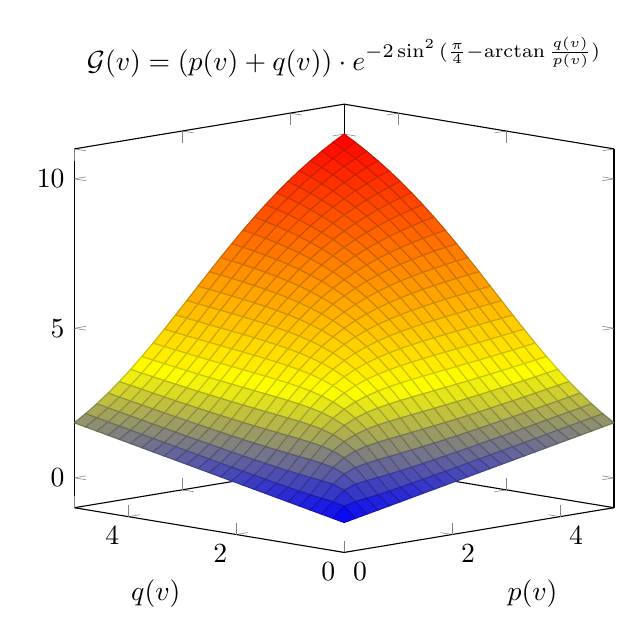
\begin{tikzpicture}[
    declare function={tf(\x)=(pi/4-rad(atan(\x)));},
    declare function={func(\x,\y)=sin(tf(\y/\x)*180/pi);}
]
\begin{axis}[
    view={315}{10},
    title={$
\mathcal{G}(v) = (p(v) + q(v)) \cdot e^{-2\sin^2{(\frac{\pi}{4} -
\arctan\frac{q(v)}{p(v)})}}$},
    xlabel=$p(v)$,
    ylabel=$q(v)$,
]

\addplot3 [
        surf,
        domain=0:5,
        domain y=0:5,
    ] {(x+y)*exp((-2)*(func(x,y))^2)};
\end{axis}
\end{tikzpicture}

\caption{The curve of the In-and-Out degree function \label{fig-surf}}
\end{figure}

\subsection{Wilbur Function \label{sec:function}}
It would be extremely complicated to calculate Core Nebulas Rank if we consider different usage case and its properities. However, we can provide a general function for Nebulas Rank.

We define the Core Nebulas Rank calculation function as \(f(x)\), namely \emph{Wilbur Function}\footnote{The name \emph{Sybil Attack} derives from 1970's TV mini-series Sybil, in which an young woman is diagnosed as suffering from muliple personalities and receives treatment from psychiatrist named Dr. Cornelia Wilbur.},where \(x\) is the factor of Core Nebulas Rank, it can be account stake, coinage or the in-and-out degree. $f(x)$ satisfies flowing two properties:

\begin{property}
\label{prop:one}
For any two variables $x_1$ and $x_2$, which are both larger than $0$, the sum of the two functions is smaller than the function of sum of two variables.
%对于任意输入$x$,将其拆分后的计算函数之和小于原计算函数。
\end{property}

\begin{align}
f(x_1+x_2)>f(x_1)+f(x_2) \quad x_1>0,x_2>0
\end{align}

\begin{property}
\label{prop:two}
For any two variables $x_1$ and $x_2$ are infinity, the sum of the two functions is approximately equal to the function of the sum of the two variables.
\end{property}

\begin{align}
\lim\limits_{x_1 \to \infty, x_2\to \infty} f(x_1+x_2) = f(x_1) + f(x_2)\quad x_1>0, x_2>0
\end{align}

These properties described above ensure, under given transaction behaviors, the benefits of splitting stakes into smaller accounts is smaller than keep them in single account. At same time, when the stake is larger enough, the cost of splitting the stakes into small accounts can be ignored. 

There is more than one function that satisfies the two properties above. Here, we provide a succinct function, the curve of the function is shown in ~\reffig{fig-nr}.
\begin{align}
f(x) = x/(1 + e^{a + b\cdot x}) \quad a>1,b<0
\end{align}
\noindent {Detailed proofs for the function are given in Appendix~\ref{sec:appendix_proof}}

\begin{figure}
\centering
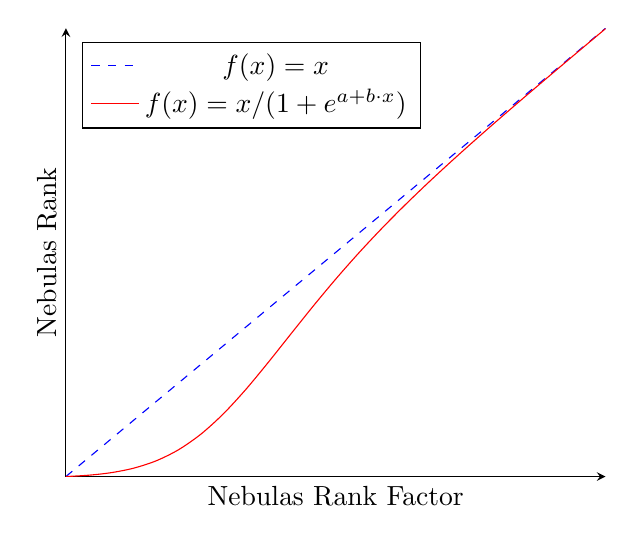
\begin{tikzpicture}[
    declare function={func(\x,\mu) = (\x / (1 + exp(\mu-\x)));},
    declare function={linefunc(\x) = \x;}
]
\begin{axis}[
    axis lines=left,
    enlargelimits=upper,
ticks=none,axis x line=bottom,axis y line=left,xlabel={Nebulas Rank Factor},
  ylabel={Nebulas Rank},
      legend pos=north west,
legend style={fill=none}
]
\addplot [dashed, domain=0:10, blue] {linefunc(x)};
\addplot [smooth, domain=0:10, red] {func(x,3)};
\addlegendentry{$f(x)=x$}
\addlegendentry{$f(x)=x/(1 + e^{a + b\cdot x})$}
\end{axis}
\end{tikzpicture}
\caption{The curve of the Nebulas Rank function \label{fig-nr}}
\end{figure}


\vspace{2em}
In summary, equation ~\ref{eq:rank} can be expressed further as below:

\begin{align}
\label{eq:rank-param}
\mathcal{C}(v) =  \frac{\beta(v)}{1+e^{a + b \cdot \beta(v)}} \cdot \frac{\gamma(v)}{1+e^{c + d \cdot \gamma(v)}}
\end{align}
\noindent where $a, b, c, d$ are parameters to be determined.


In order to verify the effectiveness of the function, we calculate the Core Nebulas Rank for all the accounts in Ethereum in certain period of time. We collected all the transaction records from May 1st 2017 to June 30th 2017 (block height: from 3629091 to 3955158), besides, we also collected average daily ETH token price (in USD) and transaction volumes ~\cite{coinmarketcap}.

~\reffig{fig-eth-simu} shows the trending of ETH market capitalization and Core Nebulas Rank of the Ethereum, where the black solid line indicates the market capitalization (in USD) of Ethereum, while the red solid line represents the summation of all accounts' Core Nebulas Rank based on function~\ref{eq:rank-param}.

We can see that the Core Nebulas Rank reflects the market capitalization changes of Ethereum precisely. The correlation coefficient is 0.84427, $p$ (p-value) is $4.48\times{}10^{-17}<0.001$. That means, the function ~\ref{eq:rank} shows the success in depicting the contributions of users to the economic system on chain, which demonstrates the validity of Core Nebulas Rank. 


\begin{figure}
\centering
\begin{tikzpicture}
  \begin{axis}[
  axis y line*=left,
  axis x line=none,
%ticks=none,
ylabel={Market Capitalization of Ethereum (USD) },
%xtick={0,10,20,30,40,50,60},
%xlabel={Time(Day)}
legend style={fill=none}
    ]
\addplot[smooth, mark=., color=red] table [x=day, y=nr, col sep=comma]
    {../common/eth_simu.csv};
\label{plot_one}

\end{axis}
  \begin{axis}[
%ticks=none,
legend pos=north west,
%ylabel={Nebulas Rank},
xlabel={Time (day) },
xtick={0,10,20,30,40,50,60},
ytick={1,2},
axis y line*=right,
legend style={fill=none}
    ]
    \addlegendimage{/pgfplots/refstyle=plot_one}\addlegendentry{Nebulas Rank}

    \addplot[smooth, mark=x] table [x=day, y=cap, col sep=comma]
    {../common/eth_simu.csv};
    \label{plot_two}
      \addlegendentry{ETH Market Cap.}
\end{axis}

\end{tikzpicture}
\caption{The market capitalization and Core Nebulas Rank of Ethereum}
\label{fig-eth-simu}
\end{figure}


